% Propósito: comparar qué estímulo ingresa, qué sensor registra la respuesta y
% qué magnitud informa una OEA frente a un PEAT.
% Origen: secciones \ref{sec:u8-oea}, \ref{sec:u8-pea} y párrafo
% "OEA y potenciales: mediciones complementarias". Esquema funcional sin
% tiempos, amplitudes, umbrales ni datos de pacientes.
% Descripción accesible: dos cadenas horizontales comienzan con un estímulo
% acústico. En la cadena OEA, una sonda emite el estímulo, el sonido atraviesa
% oído externo y medio, llega a la cóclea y una respuesta acústica regresa a un
% micrófono en el conducto; el resultado es presión o nivel y relación
% señal--ruido. En la cadena PEAT, un transductor entrega el estímulo, la
% actividad atraviesa cóclea, nervio y tronco; electrodos de superficie
% registran voltaje en microvoltios frente a tiempo en milisegundos.
% Validación prevista: comprobar la dirección de ida y retorno de OEA, que PEAT
% no muestre un micrófono como sensor, las unidades Pa/dB SPL/dB y microvoltios
% frente a milisegundos, que todos los bloques queden separados por flechas
% orientadas de manera inequívoca y la legibilidad al ancho de página.
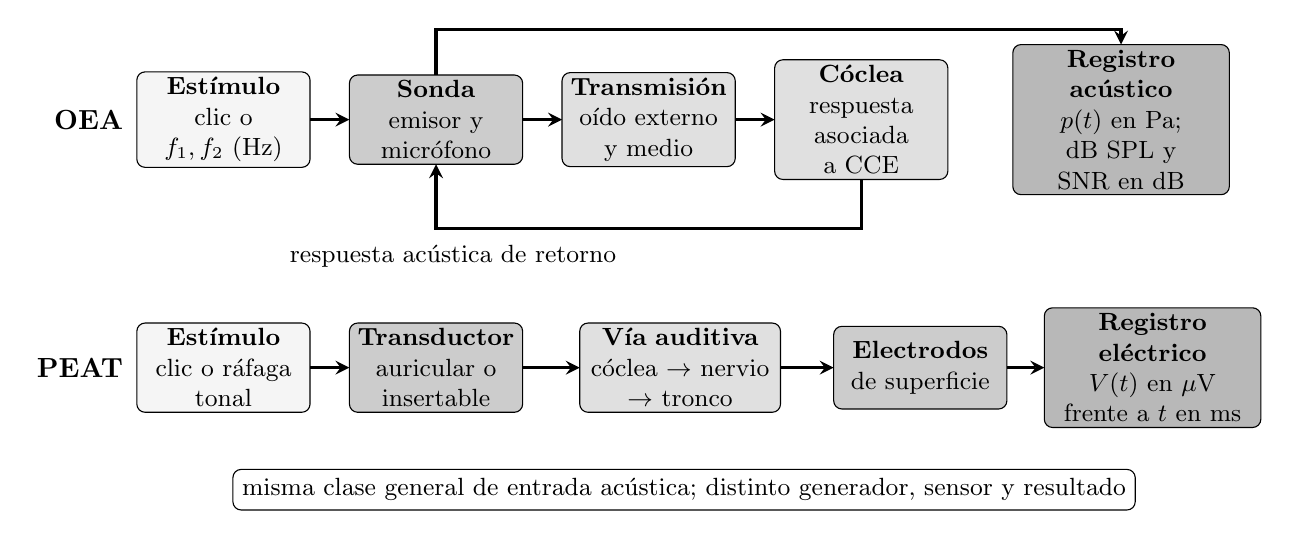
\begin{tikzpicture}[font=\small,>=stealth,x=1cm,y=1cm]
    \tikzset{
        block/.style={
            draw,rounded corners=3pt,
            text width=2.00cm,minimum width=2.20cm,minimum height=1.05cm,
            inner sep=2pt,outer sep=0pt,align=center
        },
        stimulus/.style={block,fill=black!4},
        pathway/.style={block,fill=black!12},
        sensor/.style={block,fill=black!20},
        result/.style={block,fill=black!28,text width=2.55cm,minimum width=2.75cm},
        flow/.style={->,very thick}
    }

    \node[font=\bfseries,anchor=east] at (0.00,4.40) {OEA};
    \node[stimulus] (oea-stim) at (1.15,4.40)
        {\textbf{Estímulo}\\clic o\\\(f_1,f_2\) (Hz)};
    \node[sensor] (probe) at (3.85,4.40)
        {\textbf{Sonda}\\emisor y\\micrófono};
    \node[pathway] (middle) at (6.55,4.40)
        {\textbf{Transmisión}\\oído externo\\y medio};
    \node[pathway] (cochlea) at (9.25,4.40)
        {\textbf{Cóclea}\\respuesta\\asociada a CCE};
    \node[result] (oea-out) at (12.55,4.40)
        {\textbf{Registro acústico}\\\(p(t)\) en Pa;\\dB SPL y SNR en dB};

    \draw[flow] (oea-stim.east) -- (probe.west);
    \draw[flow] (probe.east) -- (middle.west);
    \draw[flow] (middle.east) -- (cochlea.west);
    \draw[flow]
        (cochlea.south) -- ++(0,-0.62) -| (probe.south)
        node[pos=0.48,below=2pt] {respuesta acústica de retorno};
    \draw[flow] (probe.north) -- ++(0,0.58) -| (oea-out.north);

    \node[font=\bfseries,anchor=east] at (0.00,1.25) {PEAT};
    \node[stimulus] (abr-stim) at (1.15,1.25)
        {\textbf{Estímulo}\\clic o ráfaga\\tonal};
    \node[sensor] (earphone) at (3.85,1.25)
        {\textbf{Transductor}\\auricular o\\insertable};
    \node[pathway,text width=2.35cm,minimum width=2.55cm]
        (neural-path) at (6.95,1.25)
        {\textbf{Vía auditiva}\\cóclea \(\rightarrow\) nervio\\
         \(\rightarrow\) tronco};
    \node[sensor] (electrodes) at (10.00,1.25)
        {\textbf{Electrodos}\\de superficie};
    \node[result] (abr-out) at (12.95,1.25)
        {\textbf{Registro eléctrico}\\\(V(t)\) en \(\mathrm{\mu V}\)\\
         frente a \(t\) en \(\mathrm{ms}\)};

    \draw[flow] (abr-stim.east) -- (earphone.west);
    \draw[flow] (earphone.east) -- (neural-path.west);
    \draw[flow] (neural-path.east) -- (electrodes.west);
    \draw[flow] (electrodes.east) -- (abr-out.west);

    \node[draw,rounded corners=3pt,fill=white,align=center]
        at (7.00,-0.30)
        {misma clase general de entrada acústica; distinto generador,
         sensor y resultado};
\end{tikzpicture}
